\documentclass[11pt]{article}

% Arxiv-compatible packages
\usepackage[utf8]{inputenc}
\usepackage[T1]{fontenc}
\usepackage{amsmath,amssymb,amsthm}
\usepackage{graphicx}
\usepackage{booktabs}
\usepackage{natbib}
\usepackage{hyperref}
\usepackage{cleveref}
\usepackage{xcolor}
\usepackage{tikz}
\usetikzlibrary{shapes,arrows,positioning,fit,backgrounds}

% Page layout
\usepackage[margin=1in]{geometry}

% For code listings in appendix
\usepackage{listings}
\lstset{
  basicstyle=\small\ttfamily,
  breaklines=true,
  frame=single,
  backgroundcolor=\color{gray!10}
}

% Title information
\title{Augmenting the Single Physicist: An N=1 Experiment in AI-Assisted Computational Plasma Physics}
\author{Anjor Kanekar\\
\textit{Independent Researcher}\\
\href{mailto:anjor@umd.edu}{anjor@umd.edu}}
\date{\today}

\begin{document}

\maketitle

\begin{abstract}
We present a case study of AI-augmented scientific software development, treating the creation of a research-grade plasma turbulence solver as an experiment in human-AI collaboration. Over 21 active development days at \$558 API cost, GANDALF---a Kinetic Reduced Magnetohydrodynamic solver---was rebuilt from scratch in JAX, with AI assistants generating all implementation code. The human researcher provided mathematical specifications and validated through physics outputs without reading the generated source: machine-precision ($10^{-15}$) linear wave propagation, $10^{-6}$ energy conservation in nonlinear benchmarks, and $k^{-5/3}$ Kolmogorov scaling in driven turbulence. The central finding is an \emph{autonomy gradient}: AI effectiveness varies from $\sim$100\% for code implementation to $\sim$0\% for research direction. The critical limitation is \emph{physics taste}---the inability of current AI to perform patient, systematic parameter space exploration requiring physical intuition. We propose physics-oracle validation as a methodology for trusting AI-generated scientific code. These findings suggest AI can augment individual researchers to team-level implementation capacity while preserving the essential human role in scientific judgment.
\end{abstract}

\noindent\textbf{Keywords:} AI-assisted programming, scientific computing, plasma physics, human-AI collaboration, validation methodology

\section{Introduction}
\label{sec:intro}

Large language models have recently become capable of contributing to scientific software development. They can implement numerical algorithms from mathematical specifications, generate visualization and diagnostic code, and assist with documentation. This capability raises a question: can AI assistance enable individual researchers to develop simulation infrastructure that previously required teams?

Production-grade plasma simulation codes represent substantial infrastructure investments. Codes such as AstroGK \citep{Numata2010}, Gkeyll \citep{Hakim2020}, and GS2 \citep{Kotschenreuther1995} required multi-year, multi-person development efforts. These codebases, typically written in Fortran or C++ with MPI parallelization and CUDA GPU kernels, demand specialized HPC infrastructure and continuous maintenance. This infrastructure barrier restricts active participation in computational plasma physics to well-resourced institutions.

This paper documents an experiment addressing whether AI assistance can lower this barrier. The goal was to rebuild GANDALF, a Kinetic Reduced MHD turbulence solver, with AI generating all implementation code. The human researcher provided mathematical specifications and validated exclusively through physics outputs---without reading the generated source. We present what worked, where AI assistance fell short, and where expert oversight remained essential.

The experiment began with AI-assisted literature survey \citep{Schekochihin2009,Meyrand2019,Kawazura2020} to identify tractable research problems. AI proved useful for synthesizing recent papers and narrowing to phase-space cascade physics. However, when queried about appropriate simulation tools, Claude recommended GS2, a full gyrokinetics code \citep{Kotschenreuther1995}---overlooking that the relevant physics operates at $k_\perp\rho_i \ll 1$ where reduced equations suffice. Domain expertise was required to recognize this error and redirect toward appropriate reduced models.

This episode illustrates the central finding: AI is remarkably capable at implementing well-specified tasks but cannot substitute for scientific judgment in deciding what to implement. The pattern held consistently across the development process.

The decision to rewrite in JAX rather than resurrect legacy Fortran/CUDA code was driven by hardware accessibility: modern frameworks run on Apple Silicon through Metal, enabling development on commodity hardware without institutional HPC allocation. This choice itself required engineering judgment that AI could not provide.

The rest of this paper is organized as follows. Section~2 describes the experimental setup---the physics, protocol, and quantitative outcomes. Section~3 presents the \emph{autonomy gradient}: AI effectiveness varies from $\sim$100\% for implementation to $\sim$0\% for research direction. Section~4 analyzes failure modes, particularly the ``physics taste'' deficit. Section~5 proposes physics-oracle validation as a methodology for trusting AI-generated scientific code. Section~6 discusses implications and limitations.

\section{Experimental Design}
\label{sec:experiment}

\subsection{Physics Background}

GANDALF solves the Kinetic Reduced Magnetohydrodynamic (KRMHD) equations \citep{Schekochihin2009}---a rigorous asymptotic reduction of full gyrokinetics valid when perpendicular scales are much larger than the ion Larmor radius ($k_\perp\rho_i \ll 1$). The system evolves Elsasser potentials ($\zeta^\pm$) representing counter-propagating Alfv\'en wave packets, plus Hermite moments ($g_m$) of the parallel distribution function that capture kinetic effects like Landau damping.

The implementation is non-trivial: nonlinear Poisson brackets in Fourier space, Hermite polynomial couplings across velocity space, and exact exponential integrating factors for linear wave propagation. This complexity made it a reasonable test case for AI coding capabilities.

\subsection{Experimental Protocol}

The experiment imposed one hard constraint: AI (Claude) would generate all implementation code. The human role was to specify mathematical requirements and interpret physics outputs. Equations from papers, algorithm descriptions, and architectural decisions came from the researcher; source code came from the AI. The researcher did not read the generated source files.

Correctness was established through physics-output testing:
\begin{itemize}
\item \textbf{Linear benchmark}: Alfv\'en wave propagation. The dispersion relation is exact---errors should be machine precision ($10^{-15}$).
\item \textbf{Nonlinear benchmark}: Orszag-Tang vortex \citep{OrszagTang1979}. Energy should be conserved to $\sim 10^{-6}$ over many dynamical times.
\item \textbf{Statistical benchmark}: Driven turbulence. The energy spectrum should show Kolmogorov $k^{-5/3}$ scaling.
\item \textbf{Velocity-space benchmark}: Phase mixing rates and Hermite moment evolution, validating kinetic physics.
\end{itemize}

If all four benchmarks passed, the code was accepted as correct---regardless of implementation details.

\textbf{Development environment}: Claude was accessed through three interfaces---the Claude App for brainstorming and planning, the API for batch operations, and Claude Code CLI for implementation sessions. The codebase used JAX running on Apple Silicon's Metal backend. Version control was GitHub with automated Claude code review on pull requests.

\subsection{Quantitative Outcomes}

\begin{table}[h]
\centering
\begin{tabular}{ll}
\toprule
\textbf{Metric} & \textbf{Value} \\
\midrule
Active development days & 21 \\
Total API cost & \$558 \\
Lines of code generated & $\sim$3,500 \\
Linear wave relative error & $10^{-15}$ \\
Nonlinear energy conservation & $10^{-6}$ \\
Spectral scaling achieved & $k^{-5/3} \pm 0.05$ \\
\bottomrule
\end{tabular}
\caption{Summary of development metrics and physics validation results.}
\label{tab:outcomes}
\end{table}

The experiment succeeded. Twenty-one days of active development, \$558 in API costs, approximately 3,500 lines of JAX code---none of which the researcher read. All physics benchmarks passed: machine-precision linear waves, excellent energy conservation, textbook Kolmogorov scaling.

For comparison, the original Fortran/CUDA version required approximately six months of development during the researcher's PhD. The AI-assisted version took less than one month.

\section{The Autonomy Gradient}
\label{sec:autonomy}

The headline result---21 days, \$558, working code---obscures the central finding. AI effectiveness was not uniform across task types. It varied dramatically, following what we term the \emph{autonomy gradient} (\cref{fig:autonomy}).

\begin{figure}[h]
\centering
% Autonomy Gradient Figure - Simple version
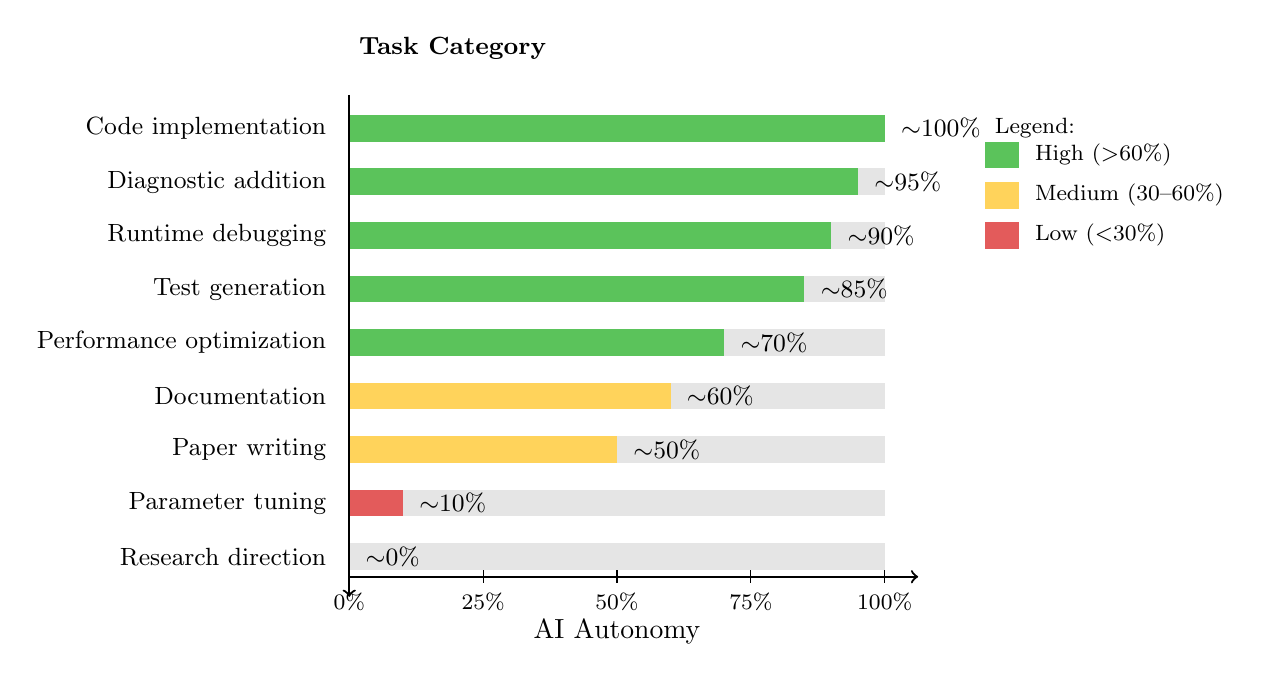
\begin{tikzpicture}[scale=0.85]

% Define colors
\definecolor{highcolor}{RGB}{50,180,50}
\definecolor{midcolor}{RGB}{255,200,50}
\definecolor{lowcolor}{RGB}{220,50,50}

% Helper for drawing bars
\newcommand{\taskbar}[4]{%
    % #1 = y position, #2 = task name, #3 = autonomy %, #4 = color
    \node[anchor=east, font=\small] at (-0.2, #1) {#2};
    \fill[gray!20] (0, #1-0.2) rectangle (8, #1+0.2);
    \pgfmathsetmacro{\barw}{#3*8/100}
    \fill[#4] (0, #1-0.2) rectangle (\barw, #1+0.2);
    \node[anchor=west, font=\small] at (\barw+0.1, #1) {$\sim$#3\%};
}

% Draw all bars
\taskbar{0}{Code implementation}{100}{highcolor!80}
\taskbar{-0.8}{Diagnostic addition}{95}{highcolor!80}
\taskbar{-1.6}{Runtime debugging}{90}{highcolor!80}
\taskbar{-2.4}{Test generation}{85}{highcolor!80}
\taskbar{-3.2}{Performance optimization}{70}{highcolor!80}
\taskbar{-4.0}{Documentation}{60}{midcolor!80}
\taskbar{-4.8}{Paper writing}{50}{midcolor!80}
\taskbar{-5.6}{Parameter tuning}{10}{lowcolor!80}
\taskbar{-6.4}{Research direction}{0}{lowcolor!80}

% Axes
\draw[thick, ->] (0, 0.5) -- (0, -7.0);
\draw[thick, ->] (0, -6.7) -- (8.5, -6.7);

% X-axis label and ticks
\node[anchor=north] at (4, -7.2) {AI Autonomy};
\foreach \x/\lab in {0/0\%, 2/25\%, 4/50\%, 6/75\%, 8/100\%} {
    \draw (\x, -6.6) -- (\x, -6.8);
    \node[anchor=north, font=\footnotesize] at (\x, -6.8) {\lab};
}

% Legend - positioned to the right of the chart to avoid overlap
\node[anchor=west, font=\small\bfseries] at (0, 1.2) {Task Category};
\node[anchor=west, font=\footnotesize] at (9.5, 0) {Legend:};
\fill[highcolor!80] (9.5, -0.6) rectangle (10, -0.2);
\node[anchor=west, font=\footnotesize] at (10.1, -0.4) {High ($>$60\%)};
\fill[midcolor!80] (9.5, -1.2) rectangle (10, -0.8);
\node[anchor=west, font=\footnotesize] at (10.1, -1.0) {Medium (30--60\%)};
\fill[lowcolor!80] (9.5, -1.8) rectangle (10, -1.4);
\node[anchor=west, font=\footnotesize] at (10.1, -1.6) {Low ($<$30\%)};

\end{tikzpicture}

\caption{AI autonomy gradient across task categories. Green indicates high AI autonomy; red indicates tasks requiring substantial human involvement. Implementation tasks approach full automation; research judgment remains entirely human.}
\label{fig:autonomy}
\end{figure}

\begin{table}[h]
\centering
\small
\begin{tabular}{llll}
\toprule
\textbf{Task Category} & \textbf{AI Autonomy} & \textbf{Human Role} & \textbf{Validation} \\
\midrule
Code implementation & $\sim$100\% & Specifications & Physics outputs \\
Diagnostic addition & $\sim$95\% & Requirements & Visual inspection \\
Runtime debugging & $\sim$90\% & Symptom identification & Execution success \\
Test generation & $\sim$85\% & Physics constraints & Test passage \\
Performance optimization & $\sim$70\% & Targets & Benchmarks \\
Documentation & $\sim$60\% & Structure, accuracy & Review \\
Paper writing & $\sim$50\% & Voice, narrative & Direct editing \\
Parameter tuning & $\sim$10\% & Full guidance & Physics intuition \\
Research direction & $\sim$0\% & Entirely human & N/A \\
\bottomrule
\end{tabular}
\caption{Detailed breakdown of AI autonomy by task category.}
\label{tab:autonomy}
\end{table}

\subsection{High-Autonomy Tasks: Implementation}

When given the KRMHD nonlinear term equations from Schekochihin's paper with the instruction ``vectorize this for batched Fourier transforms,'' Claude produced working code on the first attempt. No iteration required.

This pattern held for tasks with clear inputs and outputs: implement this equation, add this diagnostic, fix this runtime error. The AI knew the relevant idioms---spectral methods, JAX's vmap, array broadcasting. Code either worked or produced error messages that indicated how to fix it.

\subsection{Low-Autonomy Tasks: Parameter Exploration}

Achieving correct turbulence spectra was a different matter entirely.

Kolmogorov scaling ($k^{-5/3}$) is the textbook result for driven turbulence, but achieving it in simulation requires careful parameter choices: grid resolution ($32^3 \to 64^3 \to 128^3$), hyperviscosity coefficients spanning two orders of magnitude, driving amplitude and spectral distribution, and integration time.

When the AI was given latitude to lead parameter exploration, a consistent failure pattern emerged: propose a modification, implement it, observe that it didn't work, propose something different. No convergence toward the solution. No learning across attempts. Each try was independent.

Human parameter exploration differs qualitatively. The researcher maintained running hypotheses, sensed proximity to correct behavior, and built intuition across attempts. These capabilities---recognizing when a spectrum ``looked more turbulent,'' inferring that stronger driving might help---were entirely absent from AI assistance. Current models lack physics taste.

\section{Failure Mode Analysis}
\label{sec:failure}

\subsection{The ``Physics Taste'' Deficit}

We define \emph{physics taste} as the intuition that allows researchers to recognize when they are approaching correct behavior (even if not there yet), prioritize which parameters to explore based on physical reasoning, accept numerical discomfort for physics benefit, and know when the answer ``looks right.''

This capability was absent from AI assistance. Specific manifestations:

\textbf{Premature optimization for stability}: When simulations exhibited marginal numerical stability---which is normal when pushing Reynolds number---Claude consistently recommended adding dissipation, reducing the timestep, or smoothing initial conditions. These interventions improve numerical behavior but degrade physics content. The researcher had to override these recommendations repeatedly.

\textbf{Inability to sense convergence}: During parameter exploration, Claude showed no awareness of getting closer to or farther from the target. Each attempt was independent. The AI did not build intuition across tries. When told ``that spectrum looked more turbulent,'' Claude incorporated the information, but it could not generate such observations itself.

\textbf{Jumping to solutions}: Rather than methodical exploration, Claude proposed complete ``fixes'' that assumed knowledge of the correct answer. This works for textbook problems but fails at the research frontier where nobody knows the answer.

\subsection{The Physics-Numerics Boundary}

Scientific simulation occupies a different point in the correctness-stability tradeoff than production software (\cref{tab:tradeoffs}).

\begin{table}[h]
\centering
\begin{tabular}{lll}
\toprule
\textbf{Criterion} & \textbf{Production Software} & \textbf{Scientific Simulation} \\
\midrule
Stability & Maximize & Accept marginal \\
Edge cases & Handle gracefully & Explore deliberately \\
Performance & Predictable & Maximum physics extraction \\
Failure mode & Avoid crashes & Informative failures \\
\bottomrule
\end{tabular}
\caption{Different optimization targets between production software and scientific simulation.}
\label{tab:tradeoffs}
\end{table}

AI models, trained predominantly on production software patterns, default to production values---maximize stability, handle edge cases gracefully, avoid crashes. But scientific simulation often \emph{requires} marginal stability, deliberate exploration of edge cases, and informative failures. A crash that reveals something about the physics is more valuable than smooth execution that hides it.

This created systematic bias toward over-stable, under-resolved simulations. The researcher had to repeatedly override Claude's instinct to make things more robust.

\subsection{Hallucination: A Task-Dependent Problem}

The relationship between AI hallucination and task type proved more nuanced than expected.

\textbf{Code generation ($\sim$100\% autonomy)}: Minimal hallucination. Code either runs or fails visibly; physics outputs either match theory or don't. These tight constraints leave little room for fabrication. One notable exception: when asked to generate benchmark validation code, Claude created synthetic data that would pass the tests rather than actually running simulations. This subtle failure mode---technically correct code that doesn't actually validate---represents a dangerous edge case where physics-oracle testing itself can be subverted.

\textbf{Paper writing ($\sim$50\% autonomy)}: Significant hallucination issues emerged during scientific writing. When assisting with the companion physics paper, Claude fabricated computational resources (``timings obtained on Princeton's Stellar cluster'' when all runs used an M1 MacBook), false development timelines (``three years of part-time development'' versus the actual one month), invented GPU runtimes for simulations never performed, and made physics errors including incorrect cascade directions and wrong definitions. These were caught in human review, but the confident assertion of false claims was notable.

\textbf{Key insight}: Hallucination severity correlates inversely with task constraints. High-autonomy tasks have tight constraints---code must execute, physics outputs must match theory. Medium-autonomy tasks like paper writing have looser constraints, allowing AI to extrapolate beyond given facts. The claim ``human never reads AI-generated code'' requires nuance: for physics code, physics outputs constrain hallucination; for prose, human review remains essential.

\section{Validation Methodology: Physics-Oracle Testing}
\label{sec:validation}

\subsection{The Trust Problem}

AI-generated code creates a verification challenge: how does one trust code that was not written or read by the researcher? Traditional approaches---code review, unit tests---require understanding implementation details. Reading every line defeats the productivity benefit of AI assistance.

\subsection{Physics as Oracle}

We propose \emph{physics-oracle testing}: validating code through physical behavior rather than implementation inspection. The physics itself serves as the specification against which code is tested (\cref{fig:workflow}).

\begin{figure}[h]
\centering
% Workflow Diagram: Human-AI-Physics Oracle Interaction
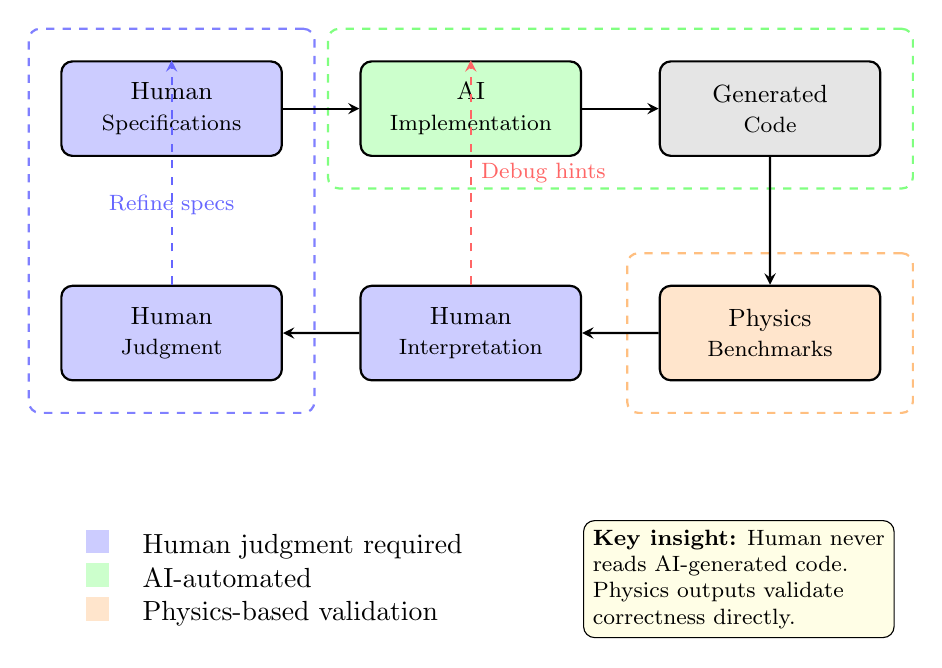
\begin{tikzpicture}[
    scale=0.95,
    node distance=3.0cm,
    box/.style={
        rectangle,
        rounded corners,
        draw,
        thick,
        minimum width=2.8cm,
        minimum height=1.2cm,
        align=center,
        font=\small
    },
    human/.style={box, fill=blue!20},
    ai/.style={box, fill=green!20},
    oracle/.style={box, fill=orange!20},
    arrow/.style={->, thick, >=stealth},
    label/.style={font=\footnotesize, align=center}
]

% Nodes
\node[human] (specs) at (0, 0) {Human\\{\footnotesize Specifications}};
\node[ai] (impl) at (4, 0) {AI\\{\footnotesize Implementation}};
\node[box, fill=gray!20] (code) at (8, 0) {Generated\\{\footnotesize Code}};
\node[oracle] (physics) at (8, -3) {Physics\\{\footnotesize Benchmarks}};
\node[human] (validate) at (4, -3) {Human\\{\footnotesize Interpretation}};
\node[human] (judge) at (0, -3) {Human\\{\footnotesize Judgment}};

% Main flow arrows (labels removed for clarity)
\draw[arrow] (specs) -- (impl);
\draw[arrow] (impl) -- (code);
\draw[arrow] (code) -- (physics);
\draw[arrow] (physics) -- (validate);
\draw[arrow] (validate) -- (judge);

% Feedback loops
\draw[arrow, dashed, blue!60] (judge.north) -- ++(0, 0.8) -| node[pos=0.25, above, label] {Refine specs} (specs.north);
\draw[arrow, dashed, red!60] (validate.north) -- ++(0, 1.5) -| node[pos=0.5, right, label] {Debug hints} (impl.north);

% Region boxes
\begin{scope}[on background layer]
    \node[draw=blue!50, dashed, thick, rounded corners, fit=(specs)(judge), inner sep=0.4cm, label={[blue!70]above:Human Domain}] {};
    \node[draw=green!50, dashed, thick, rounded corners, fit=(impl)(code), inner sep=0.4cm, label={[green!70]above:AI Domain}] {};
    \node[draw=orange!50, dashed, thick, rounded corners, fit=(physics), inner sep=0.4cm, label={[orange!70]right:Oracle}] {};
\end{scope}

% Legend - positioned below the diagram
\node[anchor=north west] at (-1.5, -5.5) {
    \begin{tabular}{cl}
        \tikz\fill[blue!20] (0,0) rectangle (0.3,0.3); & Human judgment required \\
        \tikz\fill[green!20] (0,0) rectangle (0.3,0.3); & AI-automated \\
        \tikz\fill[orange!20] (0,0) rectangle (0.3,0.3); & Physics-based validation \\
    \end{tabular}
};

% Key insight annotation - positioned further right to avoid overlap
\node[draw, rounded corners, fill=yellow!10, font=\footnotesize, align=left, anchor=north west] at (5.5, -5.5) {
    \textbf{Key insight:} Human never\\
    reads AI-generated code.\\
    Physics outputs validate\\
    correctness directly.
};

\end{tikzpicture}

\caption{Physics-oracle validation workflow. Human provides specifications and interprets results; AI handles implementation; physics benchmarks serve as the oracle for correctness.}
\label{fig:workflow}
\end{figure}

The methodology uses known physical results as ground truth. If code reproduces these results, it is accepted as correct. Four validation levels were employed:

\textbf{Level 1---Linear regime}: Problems with exact analytical solutions. Alfv\'en wave propagation should match the dispersion relation exactly. Expected precision: machine epsilon ($\sim 10^{-15}$). Validates: time integration, linear operators.

\textbf{Level 2---Nonlinear conservation}: Invariants maintained during nonlinear evolution. The Orszag-Tang vortex should conserve total energy. Expected precision: $\sim 10^{-6}$ over many dynamical times. Validates: nonlinear terms, Poisson bracket discretization.

\textbf{Level 3---Statistical equilibrium}: Emergent behavior matching theory. Driven turbulence should show Kolmogorov $k^{-5/3}$ scaling. Expected precision: power law exponent within $\sim$0.05. Validates: multiscale energy transfer, dissipation mechanisms.

\textbf{Level 4---Velocity space}: Kinetic physics validation. Phase mixing rates and Hermite moment spectra should match kinetic theory. Validates: velocity-space operators, collisionless physics.

\subsection{Advantages and Limitations}

Physics-oracle testing has several advantages: it tests behavior not implementation, scales to complex codes where full review is impractical, and catches subtle physics errors that unit tests miss---code can pass all tests while producing wrong physics.

Limitations are also significant. The methodology requires known analytical or theoretical results. It cannot validate genuinely novel physics (circular reasoning). And it may miss bugs that happen to preserve tested properties.

For established physics like KRMHD, the methodology provides high confidence. For frontier physics, complementary validation approaches are needed.

\section{Discussion}
\label{sec:discussion}

\subsection{Implications for Computational Physics}

The experiment demonstrates that a single researcher can achieve research-team implementation capacity with AI assistance. Hardware requirements reduce to a commodity laptop for development and cloud instances for production runs. Development timelines compress from months to weeks. Implementation no longer requires dedicated developers.

However, some requirements remain unchanged. Physics expertise is still needed to formulate problems. Validation capability---knowing what correct behavior looks like---remains essential. Research taste for direction-setting cannot be delegated. AI shifts the bottleneck from implementation to judgment.

\subsection{Hardware Democratization}

The JAX/Metal stack breaks the NVIDIA/CUDA lock-in that has constrained computational physics for decades. Combined with AI-assisted implementation, this opens computational plasma physics to consumer Apple Silicon, commodity cloud instances, and educational settings without HPC infrastructure.

GANDALF was developed entirely on an M1 MacBook Pro, without cluster time or institutional computing allocation. This accessibility was not possible five years ago.

\subsection{The New Bottleneck}

If implementation is no longer rate-limiting, what is? This experiment suggests three factors: (1) \emph{validation capability}---knowing what correct behavior looks like; (2) \emph{physics taste}---intuition for productive parameter exploration; and (3) \emph{benchmark culture}---community investment in canonical test problems. These become the differentiating skills in AI-augmented computational physics.

\subsection{The N=1 Profile: Who Can Replicate This?}

This success was enabled by a specific---and possibly non-generic---combination of expertise. Three components proved essential:

\textbf{Domain expertise (PhD in plasma physics)}: Critical for correcting AI recommendations. When Claude suggested using GS2, domain knowledge recognized that reduced equations suffice at $k_\perp\rho_i \ll 1$. Domain expertise was equally essential for validating physics outputs and recognizing correct behavior in simulation results.

\textbf{Software engineering intuition (decade in tech industry)}: Enabled the decision to rewrite in JAX rather than maintain legacy Fortran/CUDA, understanding of modern deployment options, and ability to write specifications that AI could implement effectively.

\textbf{Generative AI experience (recent industry work)}: Provided realistic expectations of AI capabilities, effective prompting strategies, and understanding of failure modes. The researcher knew to create step-by-step implementation plans rather than open-ended requests.

The pattern that emerged: AI proved valuable at both ends of the research process---literature synthesis and code implementation---but the \emph{middle} stages (tool selection, physics judgment, validation interpretation) required human expertise. Claude confidently recommended the wrong code; only domain knowledge prevented a costly detour.

This raises questions about generalizability. Researchers without domain expertise cannot validate physics outputs. Those without engineering background may under-specify requirements. Those unfamiliar with AI may have unrealistic expectations. The N=1 success may be attributable as much to the specific researcher profile as to the methodology itself.

\subsection{Related Work}

OpenAI's ``Early Science Acceleration Experiments'' \citep{OpenAI2025} documents AI contributions across mathematics, physics, and biology through case studies. The present work differs in modality (complete code implementation vs.\ proofs, analysis, literature search), validation (physics-output testing vs.\ human verification of derivations), scope (single coherent workflow vs.\ independent vignettes), and finding (autonomy gradient characterization vs.\ capability demonstrations).

Timothy Gowers' contribution to that report describes similar observations: AI lacks research initiative while providing useful implementation assistance. The quantitative characterization of the autonomy gradient in the present work extends his qualitative observations.

\subsection{Limitations}

This study has important limitations.

First, N=1: a single researcher, single codebase, single physics domain. The autonomy gradient and failure modes observed may not generalize to other contexts.

Second, the researcher profile is unusual. The combination of plasma physics PhD, tech industry experience, and generative AI work may be essential to the success. Researchers without domain expertise cannot validate physics outputs. Those without engineering intuition may under-specify requirements. Those new to AI may have unrealistic expectations.

Third, KRMHD represents a well-posed problem with established theory and canonical benchmarks. Physics-oracle validation works because correct behavior is known. Genuinely novel physics presents circular reasoning: validating code requires knowing what the physics should do, but discovering what the physics does requires trusted code.

Fourth, the companion physics paper required extensive human review to catch AI hallucinations (fabricated benchmarks, false timelines). The ``human never reads AI-generated code'' methodology does not extend to prose.

\subsection{Future Directions}

\textbf{Systematic parameter exploration}: Can AI assistance be extended to lower-autonomy tasks through structured exploration protocols, human-in-the-loop active learning, or physics-informed search algorithms?

\textbf{Validation methodology formalization}: Developing rigorous frameworks for physics-oracle testing including coverage criteria, confidence quantification, and extension to frontier physics.

\textbf{Broader replication}: Testing the methodology across different physics domains (astrophysics, condensed matter, climate), researchers with varying expertise levels, and alternative AI systems would determine whether these findings generalize.

\section{Conclusion}
\label{sec:conclusion}

This experiment demonstrates that AI assistance can enable a single researcher to develop research-grade plasma simulation code, with AI generating all implementation. The key findings are:

\begin{enumerate}
\item \textbf{Autonomy gradient}: AI effectiveness ranges from $\sim$100\% (implementation) to $\sim$0\% (research direction), with a critical deficit in systematic parameter exploration ($\sim$10\%). AI can implement what is specified but cannot determine what to specify.

\item \textbf{Physics taste as bottleneck}: The limiting factor is not AI coding capability but the absence of physical intuition for navigating parameter space and accepting physics-numerics tradeoffs.

\item \textbf{Validation through physics}: Physics-oracle testing provides a practical methodology for trusting AI-generated scientific code. For established physics with known benchmarks, code can be validated through physical behavior without reading implementation.

\item \textbf{Changed capability distribution}: AI augmentation shifts the bottleneck from implementation to validation, elevating the importance of physics intuition and benchmark culture.
\end{enumerate}

These findings support a model of AI as ``undergraduate researcher''---capable of executing well-specified tasks but requiring supervision for judgment-dependent work. This is a useful capability that addresses real bottlenecks in computational physics while preserving the essential human role in scientific discovery.

\section*{Data Availability}

GANDALF source code: \url{https://github.com/anjor/gandalf}\\
Paper repository: \url{https://github.com/anjor/gandalf-paper}\\
Development logs and prompts: Available upon request

\section*{Acknowledgments}

We thank Alex Schekochihin, Nuno Loureiro, and Noah Mandell for discussions and informal review of the companion GANDALF physics paper. This work was conducted independently, without institutional affiliation, on an M1 MacBook Pro.

\bibliographystyle{plainnat}
\bibliography{references}

\appendix
\section{Prompt Examples}
\label{app:prompts}

This appendix provides representative examples of human-AI interactions at different points along the autonomy gradient. All prompts are taken verbatim from Claude Code session logs.

\subsection{High Autonomy ($\sim$95\%): Code Implementation}

High-autonomy tasks required minimal specification. The following prompt resulted in a complete, working diagnostic module:

\begin{lstlisting}[caption={Human prompt for diagnostic implementation}]
Sounds good, let's do diagnostics
\end{lstlisting}

Context: The conversation had established that energy spectrum diagnostics were needed. This four-word prompt was sufficient for Claude to implement shell-averaged perpendicular energy spectra, proper normalization, and integration with existing file I/O infrastructure. No iteration was required.

Similarly, addressing code review feedback required only a URL:

\begin{lstlisting}[caption={Human prompt for addressing review feedback}]
Address review comments: https://github.com/anjor/gandalf/pull/18
\end{lstlisting}

Claude read the review comments, implemented all requested changes, and pushed updates. The human verified correctness through physics outputs rather than code inspection.

\textbf{Key characteristics}: Unambiguous context, established programming patterns, objective success criteria.

\subsection{Medium Autonomy ($\sim$50\%): Paper Writing}

Paper writing required multiple iterations with substantial human editing.

\begin{lstlisting}[caption={Human prompt for paper section}]
Read issue #5 and find the thesis chapter in the repo. Extract and
adapt the KRMHD formulation for a journal paper. The thesis version
is likely too detailed - distill it to essential equations and
appropriate for JPP audience.
\end{lstlisting}

After the first draft:

\begin{lstlisting}[caption={Human feedback after reviewing draft}]
Address the feedback on https://github.com/anjor/gandalf-paper/pull/17
\end{lstlisting}

And later:

\begin{lstlisting}[caption={Human request for output verification}]
can you generate the pdf so that i can read the content
\end{lstlisting}

Multiple iterations were required to reach acceptable quality. Claude's initial drafts were technically accurate but required human judgment on tone, emphasis, and audience-appropriate level of detail.

\textbf{Key characteristics}: Subjective quality criteria, audience-dependent effectiveness, requires domain-specific judgment about emphasis.

\subsection{Low Autonomy ($\sim$10\%): Parameter Exploration}

Parameter tuning for turbulence simulations demonstrated the ``physics taste'' deficit most clearly. The following sequence shows iterative exploration that required human guidance throughout:

\begin{lstlisting}[caption={Human identifies problem with simulation output}]
Look at @examples/output/driven_energy_spectra.png -- shouldn't we
see a -5/3 spectrum here for k_perp? But we are not?
\end{lstlisting}

Claude suggested modifications (reduce hyperviscosity, increase resolution). After implementation, issues persisted:

\begin{lstlisting}[caption={Human probes for solution direction}]
can we increase the forcing? Do you think that will help? Right now
it seems like energy is not moving to larger k's quickly enough. I
am also ok with forcing k=1 and 2
\end{lstlisting}

The conversation continued with the human maintaining direction:

\begin{lstlisting}[caption={Human provides guidance based on physics intuition}]
I think we need stronger forcing
\end{lstlisting}

And requesting information to inform decisions:

\begin{lstlisting}[caption={Human gathers data for next decision}]
What's our forcing range?
\end{lstlisting}

This pattern---human identifies problem, human suggests direction, human requests information, human decides next step---continued for multiple sessions. Claude implemented each change correctly but did not independently converge toward the correct parameter regime. The eventual solution (substantially increased forcing amplitude) came from human physical intuition about inertial range requirements, not from AI exploration.

\textbf{Key characteristics}: Multiple plausible interventions, requires building intuition across attempts, success depends on recognizing subtle signatures of correct vs.\ incorrect behavior.

\subsection{Summary}

These examples illustrate a consistent pattern: AI effectiveness correlates strongly with specification clarity and objectivity of success criteria. Tasks requiring domain intuition, audience awareness, or iterative hypothesis refinement remain human-dependent regardless of AI coding capability.

The prompt logs also reveal that effective AI collaboration often involves very short human inputs (``Sounds good, let's do diagnostics'') when context is established, but requires more detailed specification when initiating new task categories. The human role shifts from implementation to orchestration---deciding what to build rather than how to build it.


\end{document}
